\documentclass[12pt]{article}

\usepackage{fancyhdr}
\usepackage{amsthm}
\usepackage{amsmath}
\usepackage{graphicx}
\usepackage{amssymb}
\usepackage{esint}
\usepackage{subfigure}
\usepackage{color}
\usepackage{moreverb}
\usepackage{wrapfig}
\usepackage{subfig}
\usepackage{mathtools}
\usepackage{changepage}


\textwidth 17cm \topmargin -1cm \oddsidemargin 0cm \textheight 21.5cm
\pagestyle{empty} \pagestyle{fancyplain}
\lhead[\fancyplain{}{}]{\fancyplain{}{{\sc Myles Adams}}}
\chead[\fancyplain{}{}]{\fancyplain{}{{\sc CS 111 Final}}}
\rhead[\fancyplain{}{}]{\fancyplain{}{{\sc Fall 2017}}}

\newcommand{\etal}{\textit{et al. }}

\begin{document}
\centerline{\Large\textbf{CS 111 Final}}
\vspace{.5cm}

\section*{Problem 1}\label{sec::Problem1}
\subsection*{Introduction}
The goal of this first problem is to find the optimal time it takes to boil a potato. In order to do this, we will approximate the shape of a potato as a two dimensional 4cm by 5cm rectangle. At time $t_{start}=0$ a pan is filled with water and contains the potato; it is placed on the stove top. The initial temperature of the potato and water is $T_{room} = 20^\circ C$. The water temperature then quickly rises from $20^\circ c$ to $100^\circ C$ in 60 seconds and then stays at $100^\circ C$. This is modeled by the equation $T_{water} = min(20 + 80\frac{t}{60}, 100)$. Due to the thermal conduction heat propagates from water inside the potato. At the temperature of $T_{cooking} = 65^\circ C$, the cellular structure of the potato begins to change and the starch starts to gelatinize. We will assume that it takes 5 minutes (300 seconds) for the potato to fully cook once the temperature of the potato has reached the temperature $T_{cooking}$.

The temperature T = T(t,x,y) inside the potato satisfies the heat equation (diffusion equation) shown below:
\begin{center}
\begin{equation}
\frac{\partial T}{\partial t}= \lambda \Delta T ,\hspace{.3cm}(x,y) \in \Omega
\end{equation}
\end{center}
with the boundary conditions:
\begin{center}
$T(t,x,y) = T_{water}(t),\hspace{.3cm}(x,y) \in \partial \Omega$
\end{center}
and the initial conditions:
\begin{center}
$T(0,x,y) = T_{room}(t),\hspace{.3cm}(x,y) \in \partial \Omega$
\end{center}
where $\lambda$ is the thermal diffusivity constant of the potato's material. $\Omega$ and $\partial \Omega$ denote both the domain occupied in space by the potato and the boundary of this domain.
\newpage
\subsection*{Part A}
Task: Consider a generalized problem of heat transfer in a rectangle domain \Omega = $[x_{l};x_{r}]\times[y_{b};y_{t}]$
\begin{equation}
\begin{dcases}
\frac{\partial T}{\partial t} = -\lambda \Delta T + f,\hspace{2.58cm}(x,y) \in \Omega\\
T(t,x,y) = T_{bc}(t,x,y),\hspace{1.74cm}(x,y) \in \Partial \Omega\\
T(t_{start},x,y) = T_{start}(x,y),\hspace{1cm}(x,y) \in \Omega
\end{dcases}
\end{equation}
where $\lambda$ is the thermal diffusivity of the material, $f=f(t,x,y), T_{bc}(t,x,y)$ and $T_start(x,y)$ are given functions describing the source term, boundary conditions and initial conditions, respectively.

\noindent Use the \textbf{implicit} scheme to discretize (2) and explain the structure of the linear system satisfied by $\vec{T}^{n+1} = (T_{1,1}^{n+1}\hspace{.35cm}T_{1,2}^{n+1}\hspace{.35cm}...\hspace{.35cm}T_{N_{x},N_{y}}^{n+1})$.
\begin{center}
\rule{10cm}{0.4pt}
\end{center}
We will use the method of lines to choose a grid resolution $N_x$ and discretize the space as $x_1 = x_l$, $x_r = x_{N_x}$, $\Delta$ x = $\frac{x_r - x_l}{N_x - 1}$. We will do the same for y, $y_b = y_1$, $y_t = y_{N_y}$ $\Delta y = \frac{y_t - y_b}{N_y - 1}$. For time we will take $\Delta t$ = $\frac{t_{final} - t_{start}}{N_t - 1}$. We will use the backwards finite difference formula for time and the central difference formula for space. (2) will now become:
\begin{equation}
\left\{
\begin{aligned}
\frac{\partial T}{\partial t}(t_{n+1},x_i,j_j) &\approx \frac{T(t_{n+1},x_i,y_j) - T(t_n,x_i,y_j)}{\Delta t} \approx\frac{T^{n+1}_{i,j} - T^n_{i,j}}{\Delta t} \\
\frac{\partial^2 T}{\partial x^2}(t_{n+1},x_i,y_j) &\approx \frac{T(t_{n+1},x_{i+1},y_j) - 2T(t_{n+1},x_i,y_j) +T(t_{n+1},x_{i-1},y_j)}{\Delta x^2} \approx \frac{T^{n+1}_{i+1,j} - 2T^{n+1}_{i,j} + T^{n+1}_{i-1,j}}{\Delta x^2}\\
\frac{\partial^2 T}{\partial y^2}(t_{n+1},x_i,y_j) &\approx \frac{T(t_{n+1},x_i,y_{j+1}) - 2T(t_{n+1},x_i,y_j) +T(t_{n+1},x_i,y_{j-1})}{\Delta y^2} \approx \frac{T^{n+1}_{i,j+1} - 2T^{n+1}_{i,j} + T^{n+1}_{i,j-1}}{\Delta y^2}\\
\end{aligned}\right.
\end{equation}
\noindent and from this we get:
\begin{equation}
\frac{T^{n+1}_{i,j} - T^n_{i,j}}{\Delta t} = D(\frac{T^{n+1}_{i+1,j} - 2T^{n+1}_{i,j} + T^{n+1}_{i-1,j}}{\Delta x^2} + \frac{T^{n+1}_{i,j+1} - 2T^{n+1}_{i,j} + T^{n+1}_{i,j-1}}{\Delta y^2}) + f(t_{n+1},x_i,y_j)
\end{equation}
We can then use this and rearrange everything so that all unknowns are on the left side and of course, the known terms will be on the right side, giving the following:
\begin{equation}
T^{n+1}_{i,j-1}(-\frac{D\Delta t}{\Delta y^2}) + T^{n+1}_{i-1,j}(-\frac{D\Delta t}{\Delta x^2}) + T^{n+1}_{i,j}(1 + 2\frac{D\Delta t}{\Delta x^2} + 2\frac{D\Delta t}{\Delta y^2})\\
+ T^{n+1}_{i,j+1}(-\frac{D\Delta t}{\Delta y^2}) = T^n_{i,j} + \Delta t f(t_{n+1},x_i,y_j)
\end{equation}
Solving this system of equations would be much easier if is was a matrix. We will turn it into the form $A\cdot T_{n+1} = r$. We will create a column vector of grid points at the time t = $t_{n+1}$, $T_{n+1}$ as we;; as grid points at t = $t_n$ to create the column vector r.

We must now organize our grid. $T_s = T_{i,j}$ such that the index $s = (j-1)N_x + i$ for all (i,j) $\in \Omega$. The only problem now that we have is that we must modify our grid points based on if they are boundary points or not. So in order to do that, we will create a 2D matrix A which will manipulate the column vector T. For the internal points, we will follow these equations:
\begin{equation}
\begin{dcases}
r = T^n_s + \Delta t f(t_{n+1},x_i,y_j)\\
A_{s,s} = (1 + 2\frac{D\Delta t}{\Delta x^2} + 2\frac{D\Delta t}{\Delta y^2})\\
A_{s,s-1} = A_{s,s+1} = -\frac{D\Delta t}{\Delta x^2}\\
A_{s,s-N_x} = A_{s,s+N_x} = -\frac{D\Delta t}{\Delta y^2}\\
A_{s,k} = 0 \textrm{ for all other positions of the $s^{th}$ row of matrix A}
\end{dcases}
\end{equation}
Doing this will make A properly manipulate the correct values of the column vector T. We will go through all the points 1 < i < $N_x$ and 1 < j < $N_y$ and create most of A. Finally for the boundary points where i = 1 or i = $N_x$ or j = 1 or j = $N_y$ we will put the following:
\begin{equation}
\begin{dcases}
r = T_{bc}(t_{n+1},x_i,y_j) \\
A_{s,s} = 1 \\
A_{s,k} = 0 \textrm{ for all other positions of the $s^{th}$ row of matrix A}
\end{dcases}
\end{equation}

\subsection*{Part B}
Task: Implement the \textbf{implicit} scheme for solving the heat equation (2). In particular, your implementation should make a good use of the Matlab \textbf{sparse} structure. Test your code using the following example:

\hspace{4.2cm}Domain:\hspace{2.2cm} $\Omega = [-1;1] \times [-5;1.7]$

\hspace{2.15cm}Thermal diffusivity: \hspace{2cm} $\lambda = .75$

\hspace{3cm}Exact solution: \hspace{2cm} $T_{exact} = sin(x)cos(y)exp(-t)$

\noindent and where initial conditions $T_{start}(x,y)$, boundary conditions $T_{bc}(t,x,y)$ and source term $f(t,x,y)$ should be calculated from the given exact solution $T_{exact}$. Solve the heat equation (2) from $t_{start} = 0$ to $t_{final} = 1$ for grid resolutions $(N_x, N_y)$ = (25,30),(50,60) and (100,120) and time-step $\Delta t = 0.5\Delta x$. Calculate errors of numerical solutions as the maximum (among all grid points) absolute deviation from the exact solution at the moment of time $t = t_{final}$ and determine the order accuracy of the numerical method.
\begin{center}
\rule{10cm}{0.4pt}
\end{center}

In order to calculate the error in a particular trial, we use the formula:
\begin{equation*}
E = max(|T_{exact}(t_{final},x_i,y_j) - T_{i,j}^{t_{final}}|)
\end{equation*}
Once we have found the error for each trial, we can find the order of accuracy using:
\begin{equation*}
k = \left|\frac{log\left(\frac{error(trial_m)}{error(trial_{m+1})}\right)}{log(2)}\right|
\end{equation*}
We use log(2) because we are doubling $N_x$ and $N_y$ during each trial. Below, you will find a table that shows the error and order of accuracy for each resolution. From this data, it is evident that the method we are using is $1^{st}$ order accurate.
\begin{table}[htb]
\centering
\label{p1_table}
\begin{tabular}{|l|l|l|ll}
\cline{1-3}
Resolution & Error       & Order of Accuracy &  &  \\ \cline{1-3}
25 x 30    & 0.000583961 & -                 &  &  \\ \cline{1-3}
50 x 60    & 0.000278453 & 1.06844           &  &  \\ \cline{1-3}
100 x 120  & 0.000136207 & 1.03163           &  &  \\ \cline{1-3}
\end{tabular}
\caption {Error and Order of Accuracy for all resolutions}
\end{table}
\subsection*{Part C}
Task: Use your code to simulate the process of boiling a potato, that is, set parameters to
\\

\hspace{4.2cm}Domain:\hspace{2.2cm} $\Omega = [-1;1] \times [-5;1.7]$

\hspace{2.15cm}Thermal diffusivity: \hspace{2cm} $\lambda = .75$

\hspace{2.55cm}Initial conditions: \hspace{2cm} $T_{start}(x,y) = 20^\circ C$

\hspace{1.74cm} Boundary conditions: \hspace{2cm} $T_{bc}(t,x,y) = min(20 + 80\frac{t}{60}, 100)$

\hspace{3.33cm} Source term: \hspace{2cm} $f(t,x,y) = 0$
\\

Solve the heat equation from $t_{start} = 0$s to $t_{final} = 1500$s using the $N_x = 80$ grid points in the x-direction and $N_y = 100$ grid points in the y-direction and time-tep $\Delta t =$ 5s. Plot the temperature at the center of the potato ((x,y) = (0,0)) vs time and determine when this temperature reaches $T_{cooking} = 65^\circ C$. Add 300 seconds to the found time to obtain the total time needed to cook a potato. Take snapshots of the temperature distribution inside the potato at moments t = 0, 200, 400, 600 s.
\begin{center}
\rule{10cm}{0.4pt}
\end{center}
The graphs for the results are shown below. As it is shown, the time at which the potato reaches $T = 65^\circ C$ is t = 890s. Using this, the time at which the potato will be fully cooked will be 300s later at $t_{cooked} = 1190$s.

\begin{figure}[htb]%
    \centering
    {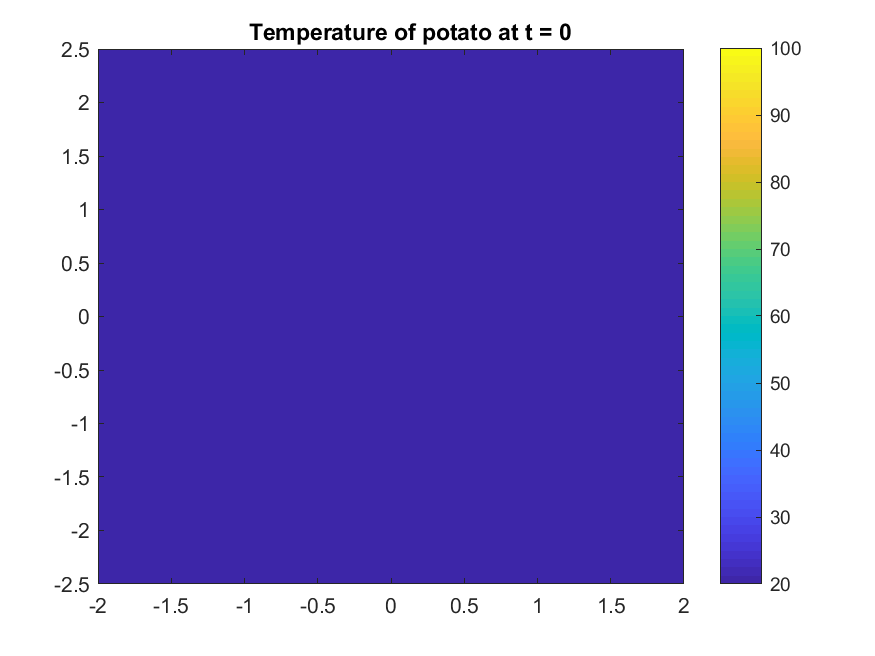
\includegraphics[width=8cm]{Problem1_fig1.png}}%
    \qquad
    {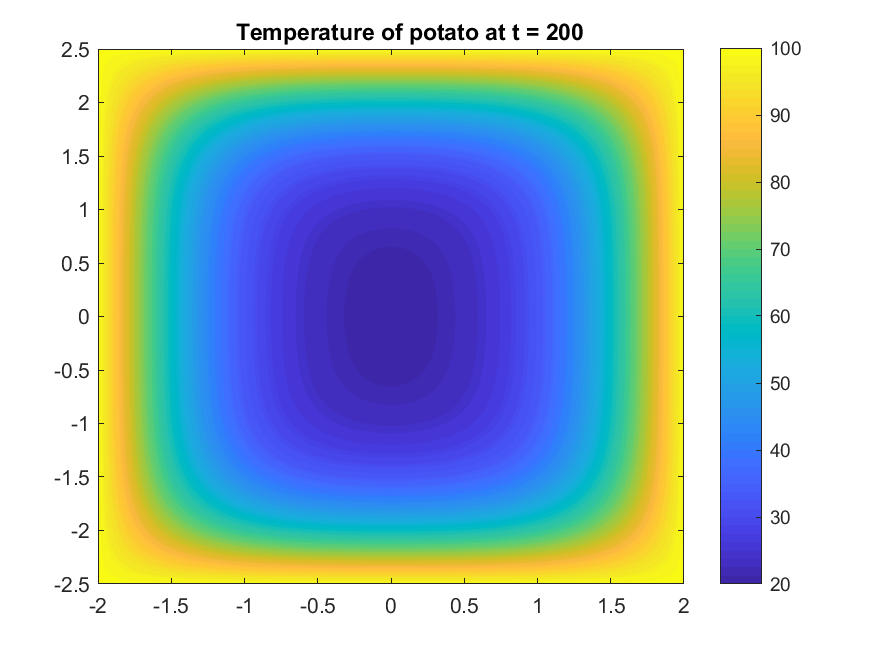
\includegraphics[width=8cm]{Problem1_fig2.png}}%
    \label{fig:p1_fig1-2}%
    \caption*{Temperature ($^{\circ}$C) throughout the potato at t = 0 and t = 200}
\end{figure}

\begin{figure}[htb]%
    \centering
    {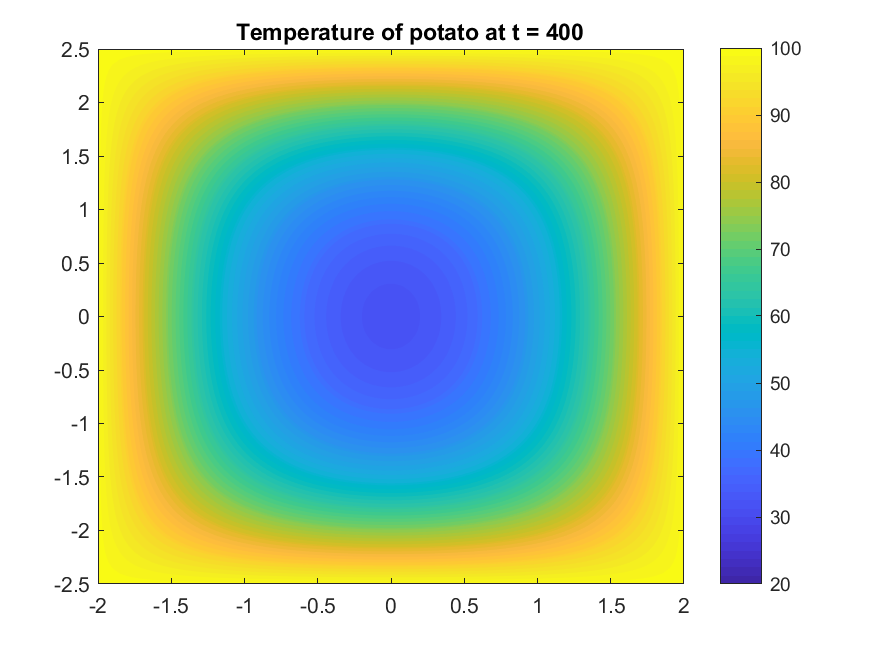
\includegraphics[width=8cm]{Problem1_fig3.png}}%
    \qquad
    {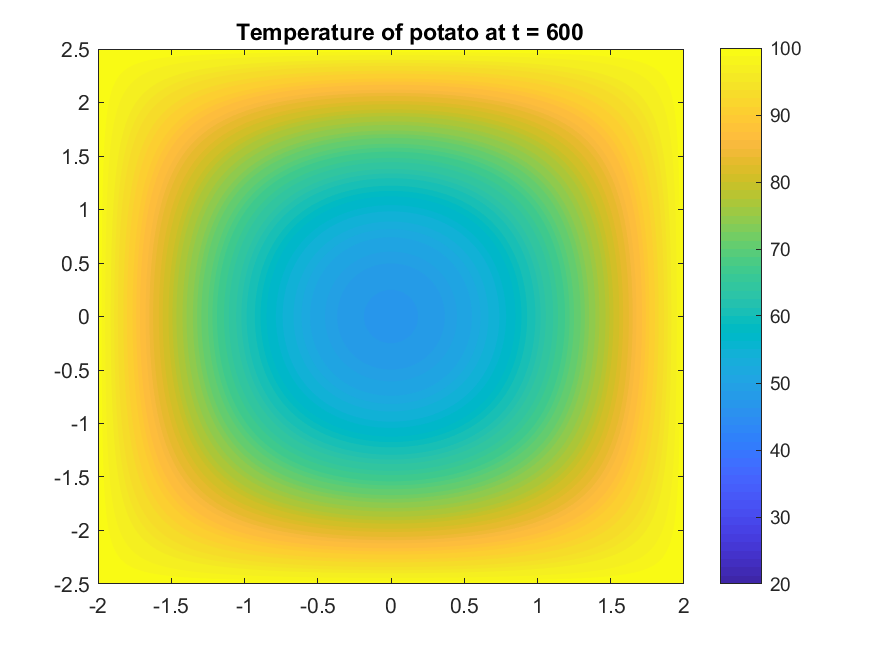
\includegraphics[width=8cm]{Problem1_fig4.png}}%
    \label{fig:p1_fig3-4}%
    \caption*{Temperature ($^{\circ}$C) throughout the potato at t = 400 and t = 600}
\end{figure}
\newpage
\vfill
\begin{figure}[]
\centering
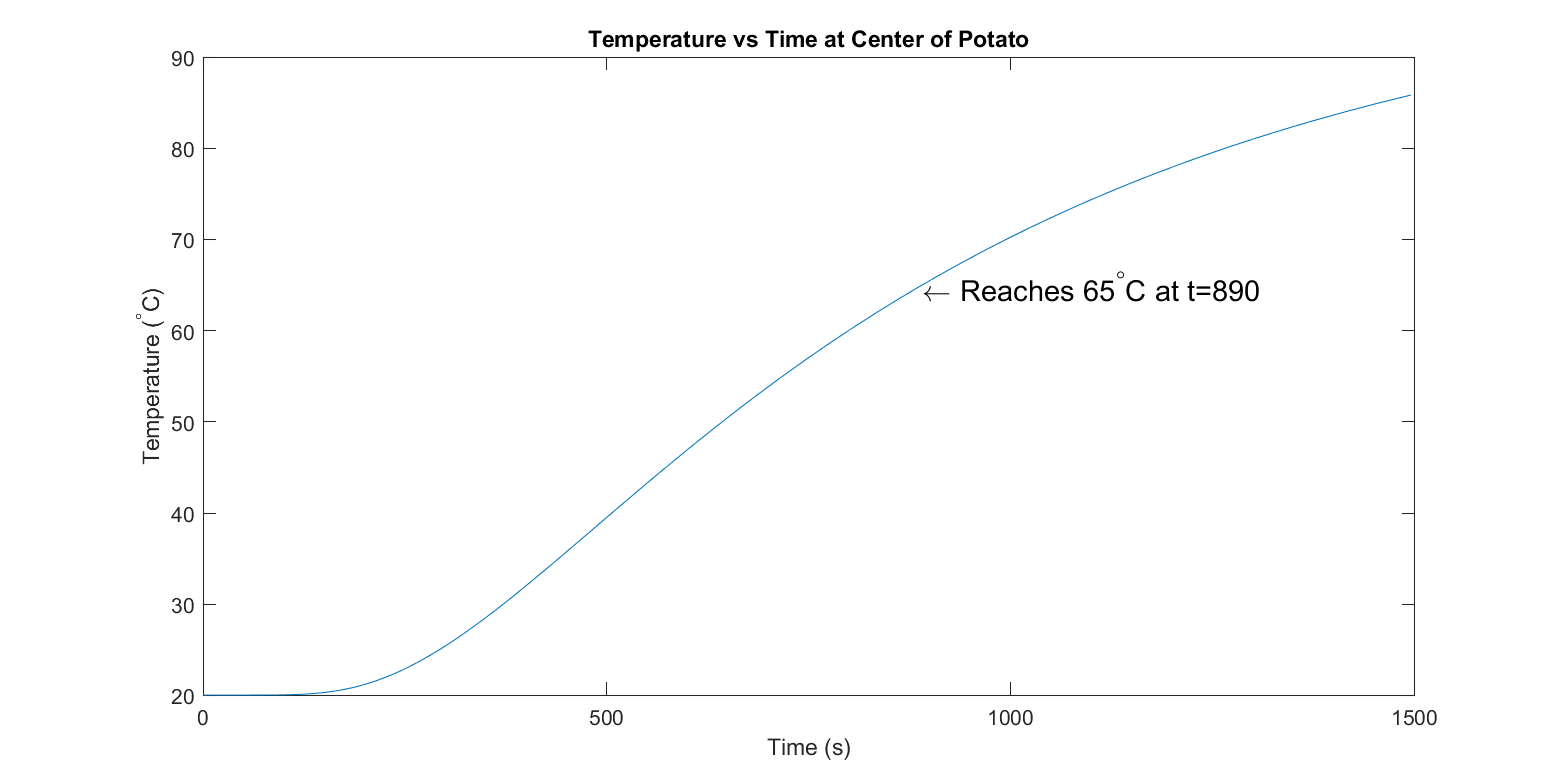
\includegraphics[width=1\textwidth]{Problem1_fig5.png}
\caption*{Temperature ($^{\circ}$C) at the center of potato vs time}
\label{fig::p1_fig5}
\end{figure}
\vfill
\clearpage

\section*{Problem 2}\label{sec::Problem2}
\subsection*{Introduction}
In this second problem we will look at a section of coastline where an oil spill has occurred. Natural diffusion and currents are the two effects causing the oil to spread in this area. We must analyze the spread of oil and the concentration in the water around three seperate beaches. We have been tasked with determining which beaches need to be closed because of unsafe levels of oil. According to the health officials, a beach where the concentration of oil is (strictly) greater than $c_{limit} = .006$ is deemed unsafe.

As an engineer, we will model this process as an advection-diffusion equation in two spatial dimensions. We will also make the assumption that the stretch of the coast we are interested in is straight. We will consider the domain $\Omega = [x_l;x_r] \times [y_b;y_t]$, a given velocity vector, $\vec{v} = \begin{pmatrix}v_{x}\\v_{y}\end{pmatrix}$, representing the ocean's currents, a source term, $f = f(t,x,y)$, which represents the amount of oil spilling into the ocean, and finally a concentration, $c = c(t,x,y)$, that represents the concentration of oil in the ocean. The concentration thus satisfies the advection-diffusion equation
\begin{equation}
\frac{\partial c}{\partial t} + \vec{v} \cdot \nabla c = D\Delta c + f, \hspace{.5cm} for\hspace{.1cm}all\hspace{.1cm} (x,y) \in \Omega
\end{equation}
\noindent where D is the rate of diffusion of oil in water, with the initial conditions
\begin{equation*}
c(t_{start},x,y) = 0.
\end{equation*}
\noindent
We will assume that the boundaries on the left, right, and top of the domain $\Omega$ are far enough, so that the oil concentration will remain zero along those boundaries during the course of the simulation.
\begin{center}
c(t,x,y) = 0, \hspace{.5cm}if $x = x_l, x = x_r,$ or $y = y_t$
\end{center}

However, the bottom boundary behaves differently. The oil concentration along this bottom boundary of $\Omega$ has to satisfy the no-flux condition:
\begin{center}
$D\frac{\partial c}{\partial y} - v_yc = 0$,\hspace{.5cm} if $y = y_b$
\end{center}
\newpage
\subsection*{Part A}
Task: Consider a generalized advection-diffusion problem in a rectangle domain $\Omega = [x_l;x_r] \times [y_b;y_t]$
\begin{equation}
\begin{dcases}
PDE:\hspace{.5cm}\frac{\partial c}{\partial t} + \vec{v} \cdot \nabla c = D\Delta c + f,\hspace{1.3cm}(x,y) \in \Omega\\
BC:\hspace{.9cm}c(t,x,y) = c_{bc}(t,x,y),\hspace{1.74cm} if \hspace{.1cm}x = x_l, x = x_r, or \hspace{.1cm}y = y_t\\
\hspace{1.85cm}D\frac{\partial c}{\partial y} - v_yc = g(t,x,y),\hspace{1.55cm}if \hspace{.1cm}y = y_b\\
IC:\hspace{1cm}c(t_{start},x,y) = c_{start}(x,y),\hspace{1cm}(x,y) \in \Omega
\end{dcases}
\end{equation}
\\
where D is the diffusivity, $f = f(t,x,y), c_{bc} = c_{bc}(t,x,y), g = g(t,x,y)$ and $c_{start} = c_{start}(x,y)$ are given functions describing the source term, boundary conditions and initial conditions.

\noindent Use the \textbf{explicit upwind} approximation to discretize the advection term $\vec{v} \cdot \nabla c$ and the \textbf{implicit} approximation to discretize the diffusion term $D\Delta c$. Explain the structure of the linear system satisfied by $\vec{c}^{n+1} = (c_{1,1}^{n+1}\hspace {.35cm}c_{1,2}^{n+1} \hspace {.35cm}... \hspace{.35cm}c_{N_{x},N_{y}}^{n+1})$.
\begin{center}
\rule{10cm}{0.4pt}
\end{center}
Much like Problem 1a, we will use the method of lines to choose a grid resolution $N_x$ and discretize the space as $x_1 = x_l$, $x_r = x_{N_x}$, $\Delta$ x = $\frac{x_r - x_l}{N_x - 1}$. We will do the same for y, $y_b = y_1$, $y_t = y_{N_y}$ $\Delta y = \frac{y_t - y_b}{N_y - 1}$. For time we will take $\Delta t$ = $\frac{t_{final} - t_{start}}{N_t - 1}$. We will apply the explicit upwind scheme to the advection terms, and for the diffusion term we will apply the implicit scheme. From this we come to the equation:
\begin{equation}
\frac{\partial c}{\partial t}(t_{n}, x_i,y_j) + (v_x\frac{\partial c}{\partial x} + v_y\frac{\partial c}{\partial y})= D \frac{\partial ^2 c}{\partial x^2} (t_{n}, x_i,y_j) + D \frac{\partial ^2 c}{\partial y^2} (t_{n}, x_i,y_j) + f (t_{n}, x_i,y_j)
\end{equation}
We will use the central-difference approximation to approximate the spacial second derivatives. And for time we will approximates its derivate using the backward difference method:
\begin{equation*}
\frac{\partial ^2 c}{\partial x^2} (t_{n+1}, x_i,y_j) \approx \frac{c^{n+1}_{i+1,j} - 2c^{n+1}_{i,j}+c^{n+1}_{i-1,j}}{\Delta x^2}
\end{equation*}
\begin{equation*}
\frac{\partial ^2 c}{\partial y^2} (t_{n+1}, x_i,y_j) \approx \frac{c^{n+1}_{i,j+1} - 2c^{n+1}_{i,j}+c^{n+1}_{i,j-1}}{\Delta y^2}
\end{equation*}
\begin{equation*}
\frac{\partial c}{\partial t} (t_{n}, x_i,y_j) \approx \frac{c_{i,j}^{n+1}-c_{i,j}^n}{\Delta t}
\end{equation*}
\begin{equation*}
(v_x\frac{\partial c}{\partial x} + v_y\frac{\partial c}{\partial y}) \approx v_x(\frac{c^n_{i+1,j} - c^n_{i,j}}{\Delta x}) + v_y(\frac{c^n_{i,j+1} - c^n_{i,j}}{\Delta y})
\end{equation*}
From this we can obtain the equation:
\begin{equation}
\hspace{-1.7cm}\frac{c_{i,j}^{n+1}-c_{i,j}^n}{\Delta t} + v_x(\frac{c^n_{i+1,j} - c^n_{i,j}}{\Delta x}) + v_y(\frac{c^n_{i,j+1} - c^n_{i,j}}{\Delta y}) = D \frac{c^{n+1}_{i+1,j} - 2c^{n+1}_{i,j}+c^{n+1}_{i-1,j}}{\Delta x^2} + D \frac{c^{n+1}_{i,j+1} - 2c^{n+1}_{i,j}+c^{n+1}_{i,j-1}}{\Delta y^2}+ f(t_{n+1}, x_i, y_j)
\end{equation}
We can use this equation for all internal grid points on our domain. For the bottom boundary condition, we will need to apply the Robin boundary conditions, because the no-flux conditions must be met by the bottom boundary. The only exception along the bottom boundary is the very right and very leftmost points because they adhere to the boundary conditions of the left and right boundaries. For the left, right, and top boundaries we apply the Dirichlet boundary condition function.

Because of the fact that, in order to solve the equation at time $t = t_{n+1}$ we must know the solution at that time, we need to create a system of equations and solve for all $N_xN_y$ equations at once. In order to do this, we will do what we did in Problem 1a, or something similar, and solve our equations using matricies. We will set it up as the problem $A\cdot x = r$ where x is the column vector for the grid points at the time $t = t_n+1$ for $c_{s}^{n+1}$. The index of s is given by the equation $s = (j-1)N_x + i\hspace{.5cm} \forall (i,j)$. Row s of A and r are constructed differently if the $s^{th}$ point is a boundary point, or internal point. For the internal grid points we will do the following:
\begin{equation}
\begin{dcases}
A_{s,s} &= 1 + 2D\Delta t(\frac{1}{\Delta x^2} + \frac{1}{\Delta y^2})\\
A_{s,s+1} &= A_{s,s-1} = -\frac{D\Delta t}{\Delta x^2}\\
A_{s,s+N_x} &= A_{s,s-N_x} = -\frac{D \Delta t}{\Delta y^2}\\
b_s &= c^n_{i,j} + \Delta t f(t_{n+1},x_i,y_j) - v_x\Delta t \frac{c^n_{i+1,j} - c^n_{i,j}}{\Delta x} - v_y\Delta t \frac{c^n_{i,j+1} - c^n_{i,j}}{\Delta y}
\end{dcases}
\end{equation}
If it is a bottom boundary point that is not also a corner point, we will apply the Robin BC as follows:
\begin{equation}
\begin{dcases}
	A_{s,s} &= 1 + 2D\Delta t(\frac{1}{\Delta x^2} + \frac{1}{\Delta y^2}) + \frac{2v_y\Delta t}{\Delta y}\\
	A_{s,s+1} &= A_{s,s-1} = -\frac{D\Delta t}{\Delta x^2}\\
	A_{s,s+N_x} &= -2\frac{D \Delta t}{\Delta y^2}\\
b_s &= c^n_{i,j} + \Delta t f(t_{n+1},x_i,y_j) - v_x\Delta t \frac{c^n_{i+1,j} - c^n_{i,j}}{\Delta x} - v_y\Delta t \frac{c^n_{i,j+1} - c^n_{i,j}}{\Delta y} -\frac{2\Delta t}{\Delta y}g(t_{n+1},x_i,y_1)
\end{dcases}
\end{equation}
Lastly, for the top, left, and right boundary conditions, we will apply the Dirichlet conditions as follows:
\begin{equation}
\begin{dcases}
	A_{s,s} &= 1\\
	b_s &= c_{bc}(t_{n+1},x_i,y_j)
\end{dcases}
\end{equation}
While we have now defined the column vectors x and r completely, we have not yet defined every single grid point of the matrix A. With the remaining points $A_{i,j}$ that have not been defined, we will set them equal to 0. Because our matrix will become very large as we start to use bigger $N_x$ and $N_y$ values and much of the A matrix is 0's, we can use the Sparse structure in MATLAB. This will speed up computation time by an incredible amount.

\subsection*{Part B}
Task: Implement the obtained numerical scheme. In particular, your implementation should make a good use of the Matlab \texbf{sparse} structure. Test your code using the following example:
\\

\hspace{4.2cm}Domain:\hspace{2.2cm} $\Omega = [-1;3] \times [-1.5;1.5]$

\hspace{2.15cm}Thermal diffusivity: \hspace{2cm} $D = .7$

\hspace{3.27cm}Velocity field: \hspace{2cm} $v_x = -0.8$

\hspace{8cm} $v_y = -0.4$

\hspace{2.88cm} Exact solution: \hspace{2cm} $c_{exact} = sin(x)cos(y)exp(-t)$
\\

\noindent and where initial conditions $c_{start}(x,y)$, boundary conditions $c_{bc}(t,x,y)$ and $g(t,x,y)$, and source term $f(t,x,y)$ should be calculated from the given exact solution $c_{exact}$. Solve the advection-diffusion equation from $t_{start} = 0$ to $t_{final} = 1$ using grid resolutions $(N_x, N_y)$ = (20,15), (40,30), (80,60), and (160,120) and time-step $\Delta t = 0.5\Delta x$. Calculate errors of numerical solutions as the maximum (among all grid points) absolute deviation from the exact solution at the moment of time $t = t_{final}$ and determine the order of accuracy of the numerical method.
\begin{center}
\rule{10cm}{0.4pt}
\end{center}
In order to calculate the error in a particular trial, we use the formula:
\begin{equation*}
E = max(|c_{exact}(t_{final},x_i,y_j) - c_{i,j}^{t_{final}}|)
\end{equation*}
Once we have found the error for each trial, we can find the order of accuracy using:
\begin{equation*}
k = \left|\frac{log\left(\frac{error(trial_m)}{error(trial_{m+1})}\right)}{log(2)}\right|
\end{equation*}
We use log(2) because we are doubling $N_x$ and $N_y$ during each trial. Below, you will find a table that shows the error and order of accuracy for each resolution. From this data, it is evident that the method we are using is $1^{st}$ order accurate.
\begin{table}[htb]
\centering
\label{p2_table}
\begin{tabular}{|l|l|l|}
\hline
Resolution & Error      & Order of Accuracy \\ \hline
20 x 15    & 0.0240409  & -                 \\ \hline
40 x 30    & 0.0119852  & 1.00424           \\ \hline
80 x 60    & 0.00598461 & 1.00193           \\ \hline
160 x 120  & 0.00299154 & 1.00037           \\ \hline
\end{tabular}
\caption{Error and Order of accuracy for each resolution}
\end{table}
\subsection*{Part C}
Task: Use your code to simulate spreading of the oil in the ocean, that is, set parameters of the problem to:
\\

\hspace{2.7cm}Domain:\hspace{1.2cm} $\Omega = [0;12] \times [0;3]$

\hspace{.65cm}Thermal diffusivity: \hspace{1cm} $D = .2$

\hspace{1.77cm}Velocity field: \hspace{1.5cm} $v_x = -0.8$

\hspace{5.5cm} $v_y = -0.4$

\hspace{1.05cm}Initial conditions: \hspace{1cm} $c_{start}(t,x,y) = 0$

\hspace{.24cm} Boundary conditions: \hspace{1cm} $c_{bc}(t,x,y) = 0$

\hspace{5.5cm} $g(t,x,y) = 0$

\hspace{1.83cm} Source term: \hspace{1cm} $f(t,x,y) = \begin{equation*}
\begin{dcases}
\frac{1}{2}\left(1-\tanh \left( \frac{\sqrt{(x-x_s)^2+y^2}-r_s}{\epsilon}\right)\right), \hspace{.5cm}if\hspace{.2cm} t<0.5\\
f(t,x,y) = 0, \hspace{.5cm}if\hspace{.2cm} t>0.5
\end{dcases}
\end{equation*}$
\\

\noindent where $x_{s} = 10, r_{s} = 0.1, \epsilon = 0.1$. Solve the advection diffusion equation from $t_{start} = 0$ to $t_{final} = 10$ using $N_x = 160$ grid points in the x-direction and $N_y = 40$ points in the y-direction and time-step $\Delta t = 0.1$. Plot the oil concentration at points (x,y) = (4,0), (6,0), (8,0) vs time and determine time periods at which each of the three beaches should be closed. Take snapshots of the oil concentration at moments of time t = 1, 4, 7.
\begin{center}
\rule{10cm}{0.4pt}
\end{center}
Below you can find the graphs that correspond to the data we were tasked to find. In the end, we can determine that all three beaches should be closed. The beach at (4,0) reached a concentration of .006 between t=5.2 and t = 5.3. The beach at (6,0) reached a concentration of .006 between t=3.2 and t=3.3. The last beach at (4,0) reached a concentration of .006 between t=1.2 and t=1.3.
\begin{figure}[htb]
\begin{adjustwidth}{-2cm}{-2cm}
\centering
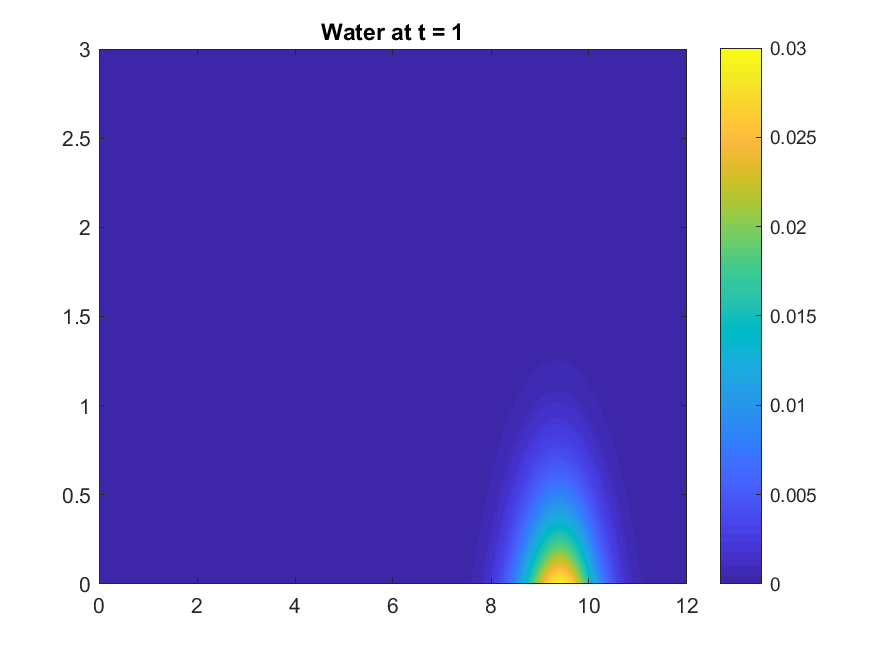
\includegraphics[width=.41\textwidth]{Problem2_fig1.png}\hfill
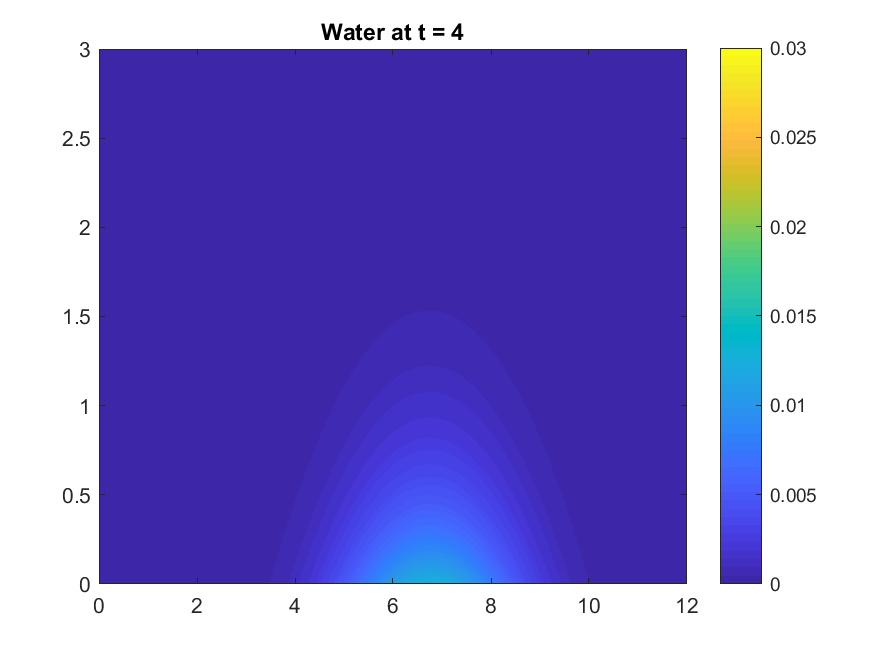
\includegraphics[width=.41\textwidth]{Problem2_fig2.png}\hfill
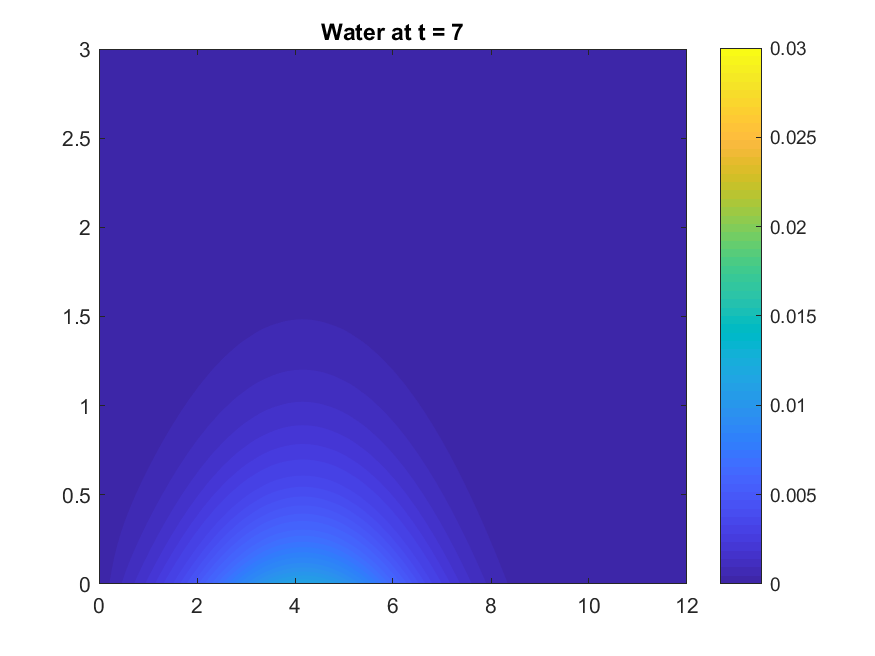
\includegraphics[width=.41\textwidth]{Problem2_fig3.png}
\caption*{Oil concentration in water at t=1, t=4, and t=7}
\label{fig:p2_fig1-3}
\end{adjustwidth}
\end{figure}

\begin{figure}[htb]
\begin{adjustwidth}{-2cm}{-2cm}
\centering
\hspace{-.9cm}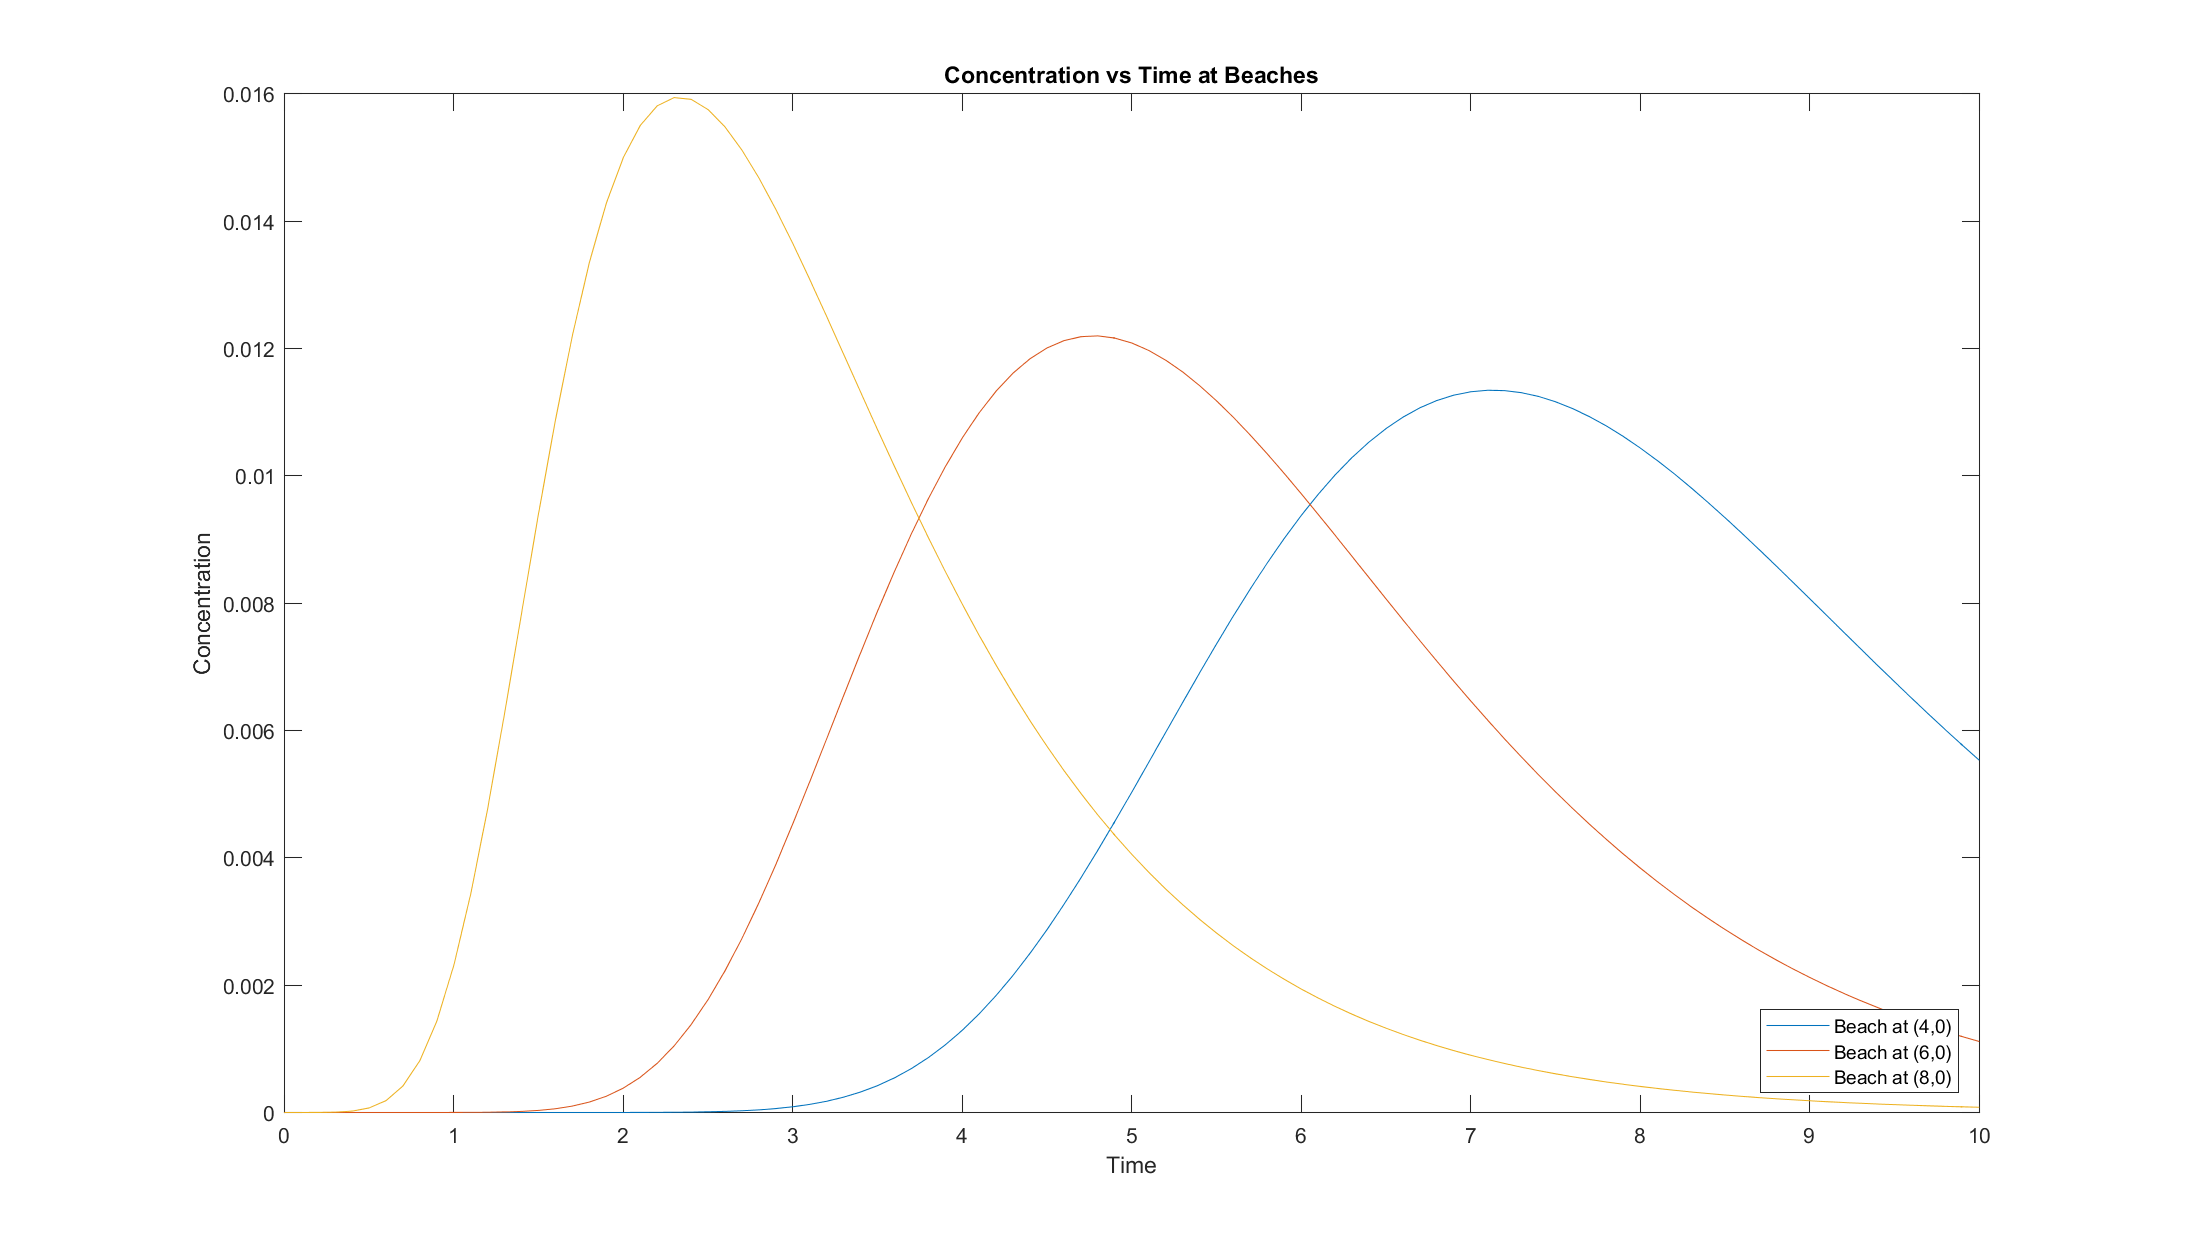
\includegraphics[width=1.2\textwidth]{Problem2_fig4.png}
\caption*{Concentration of oil at each beach vs time}
\label{fig::p2_fig5}
\end{adjustwidth}
\end{figure}


\newpage
\clearpage
\setcounter{page}{1} \pagestyle{empty}
\section*{References}\label{sec::References}
\begin{itemize}
\item [1] Daniil Bochkov, CS 111 - Introduction to Computational Science - Final, Fall 2017
\item [2] Daniil Bochkov, CS 111 - Introduction to Computational Science - Lecture 9 - Intro to PDEs, Fall 2017
\item [3] Daniil Bochkov, CS 111 - Introduction to Computational Science - Lecture 10 - Solving the Advection Equation,  Fall 2017
\item [4] Daniil Bochkov, CS 111 - Introduction to Computational Science - Lecture 11 - Solving Diffusion 1D, Fall 2017
\item [5] Daniil Bochkov, CS 111 - Introduction to Computational Science - Lecture 12 - Solving Diffusion 2D, Fall 2017
\item [6] Daniil Bochkov, CS 111 - Introduction to Computational Science - Lecture 13 - Boundary Conditions, Fall 2017
\end{itemize}
\end{document}
